\section{Experiments}


\subsection{Input data}
To test the correctness of the algorithms we used the MONK's and the ML-CUP datasets. To use these dataset correctly we did the following steps:
\begin{itemize}
	\item We preprocessed MONK's datasets with \textit{1-of-k} encoding to convert categorical data to numerical data and we obtained 17 binary input features vectors. This preprocessing is divided between two classes, \textit{Preprocessing} and \textit{LoadDataset}. The former reads, shuffle and split the dataset whereas the latter performs the \textit{1-to-k} encoding. We didn't preprocess the ML cup dataset with \textit{1-of-k} encoding since the data are already in numerical format.
	\item Since the two datasets present different model purposes we structured our library to deal with classification and regression tasks exploiting the composition of the \textit{Layer} class.  So we implemented \textit{sigmoid} and \textit{linear} activation functions for the output layer and \textit{hyperbolic tangent} activation function for the hidden layers.
	\item To view all the network in vector formulation terms and exploit the \textit{Armadillo} numerical library, we performed batch computation by loading and transposing the entire dataset in a single matrix. The labels were split and saved in another matrix to compute the \textit{MSE} (sez \ref{Loss:Mse}) after the forward phase. To reduce the cost of moving matrices we took advantage of the \textit{move} operator available since C++11. 
\end{itemize}

\subsection{Choose and describe the experimental set-up}

\begin{figure}[H]
	\centering
	\begin{minipage}[t]{0.5\linewidth}
		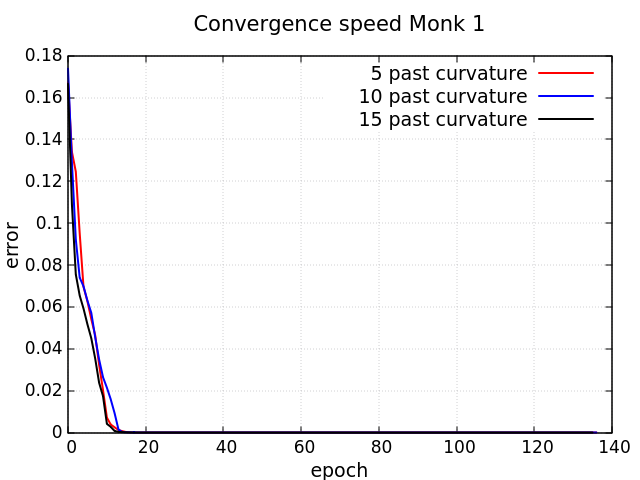
\includegraphics[width=\linewidth]{img/Monk1_LBFGS_NoReg_standard.png}
		%\subcaption{MSE}
	\end{minipage}%
	\begin{minipage}[t]{0.5\linewidth}
		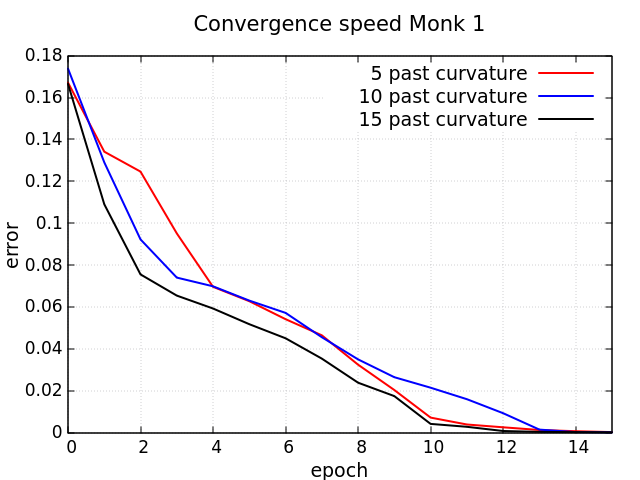
\includegraphics[width=\linewidth]{img/Monk1_LBFGS_NoReg_zoom.png}
		%\subcaption{Accuracy}
	\end{minipage}
	\caption{LBFGS convergence for MONK’s 1.}
\end{figure}
\texttt{Next, set up and describe experiments. You are supposed to test the algorithm on a realistic range of examples, interms of size, structure, and sparsity: it is typically not OK if your largest example is 10x10. While you are notexpected to fire up an HPC to run your test suite, you are welcome to try to get a sense on how algorithms scale, andwhat would be the maximum size of problems that you could successfully tackle on an ordinary machine.Numerical experiments are performed mainly for two reasons:•To confirm that the methods work as expected: how close do they get to the true solution of the problem? Howcan you check it? Is there a “residual”, or “gap” value that you can check? Do they converge with the expectedrate (linearly, sublinearly, superlinarly, . . . ) that the theory predicts? Does the error decrease monotonically, ifit is expected to do so?•To evaluate trade-offs and compare various algorithms: which algorithm is faster? If algorithm\part{title} A takes feweriterations than algorithm B, but the single iterations are more expensive, which one is the winner? How doesthis depend on the characteristics of the problem to be solved (size, density, . . . )?
3 Project submission and oral exam3Comparison with off-the-shelf algorithms is also welcome (and typically necessary at least to check correctness) toassess whether your approach could ever be competitive under the right conditions (and what these are).During this process, properly setting thresholds and algorithmic parameters is a key and completely nontrivialaspect.  Proper setting of thresholds and algorithmic parameters is indeed one of the “dark secrets” of numericalalgorithms: basically any algorithm you can write has them, and it will misbehave if you don’t set them properly.Also, their setting can have a huge impact on performamce. Thus, a minimal testing activity about the effect of theparameters is almost surely needed. A full-scale test a-la hypermetameters optimization in ML is also completelypossible, and welcome, but be aware that this is anyway rather different from what one would do in ML, even for“ML projects”. The point is that the properties one is looking at are fundamentally different: for ML one looks forlearning (accuracy, recall, . . . ), while in this course one is looking at “how close the solution I got is to what I wouldhave liked to get, and how costly was it to get there”. Hence, reporting here the same hypermetameters optimizationtables done for ML does not cut it. Not that thesecannotbe reported, as they still give some potentially interestinginformation, but it’s not the information we are crucially interested in.When designing your experiments, and later your graphs and/or tables, you should have these goals in mind. Toquote a famous mathematician, “the purpose of computing is insight, not numbers.”}

\subsection{Results}
A few plots and/or tables are required to display your results. Have a purpose in mind: as for the choice of experiments,these plots should display the important features of the algorithm: convergence speed, residual, computational time,. . .Plots should be readable. If 90\% of your plot are barely-visible horizontal or vertical lines, look for a better way todisplay information. In particular,logarithmic scalesare usually a good idea to display quantities (such as residualsor errors) that vary by orders of magnitude; use them wisely. In particular, a nice feature of logarithmic plots is thata sequence with exact linear convergence (errork+1=C·errork) becomes a straight line in a logarithmic plot; hencethey display well the convergence speed of algorithms.For “ML projects”, the quantities you want to plot may be quite different from these you would in a ML course.While the “learning rate” (here “convergence rate”) is basically the same, the out-of-sample performances of the learntsolution are much less relevant here. They can still be displayed as side information, but it’s not the core result oneshould be looking at.